Dans notre projet de classification de tweets en scientifiques et non scientifiques, nous avons appliqué trois types de classification et à chaque étape, un bon prétraitement s’est révélé indispensable pour améliorer la qualité des données et les performances des modèles.
En effet, les tweets bruts contiennent souvent du bruit (liens, hashtags, mentions, emojis, etc.), ce qui peut perturber l’apprentissage.

Nous avons donc appliqué les étapes suivantes, adaptées à chaque tâche :
\begin{itemize}
    \item Nettoyage textuel et des \textit{stop words}
    \item Normalisation linguistique : Lemmatisation et tokenisation
    \item Vectorisation avec TF-IDF et paramétrage des n-grammes
    \item Gestion du déséquilibre
\end{itemize}

Des tests ont été effectués dans le cadre de cette classification en utilisant uniquement les attributs importants extraits à l’aide du classifieur Random Forest.
Cependant, les résultats n’étaient pas très satisfaisants.
Nous avons donc envisagé de réduire manuellement la taille maximale des features lors de la vectorisation, afin d’observer le comportement du modèle.
Cette décision se justifie par la présence de bruit dans les données, bruit qui reste néanmoins représentatif pour distinguer les tweets scientifiques des non-scientifiques.
C’est pourquoi nous avons choisi de ne pas effectuer une classification uniquement à partir de ces attributs.

Ces étapes ont été adaptées à chaque type de classification (Scientifique versus Non Scientifique, Affirmation et Référence versus Contexte, Affirmation versus Référence versus Contexte) afin d’obtenir les meilleures performances.
Dans la suite de ce rapport, une comparaison entre les données brutes et les données après traitement sera présentée, accompagnée d’une justification des choix effectués.
Par la suite pour chaque classification, on effectuera une évaluation comparative (\autoref{fig:pca-bpt} et \autoref{fig:pca-apt}) des performances de classification.

\begin{figure}[H]
    \centering
    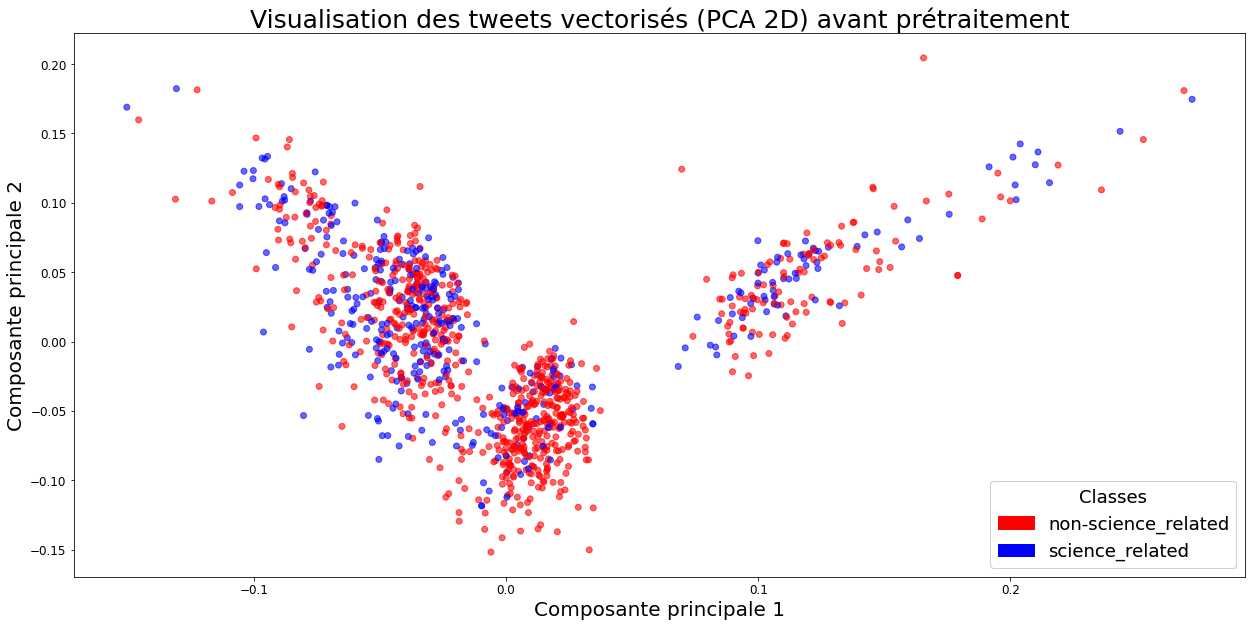
\includegraphics[width=\textwidth]{images/PCA-BPT}
    \caption{Visualisation des tweets vectorisés (PCA 2D) avant prétraitement}
    \label{fig:pca-bpt}
\end{figure}

\begin{figure}[H]
    \centering
    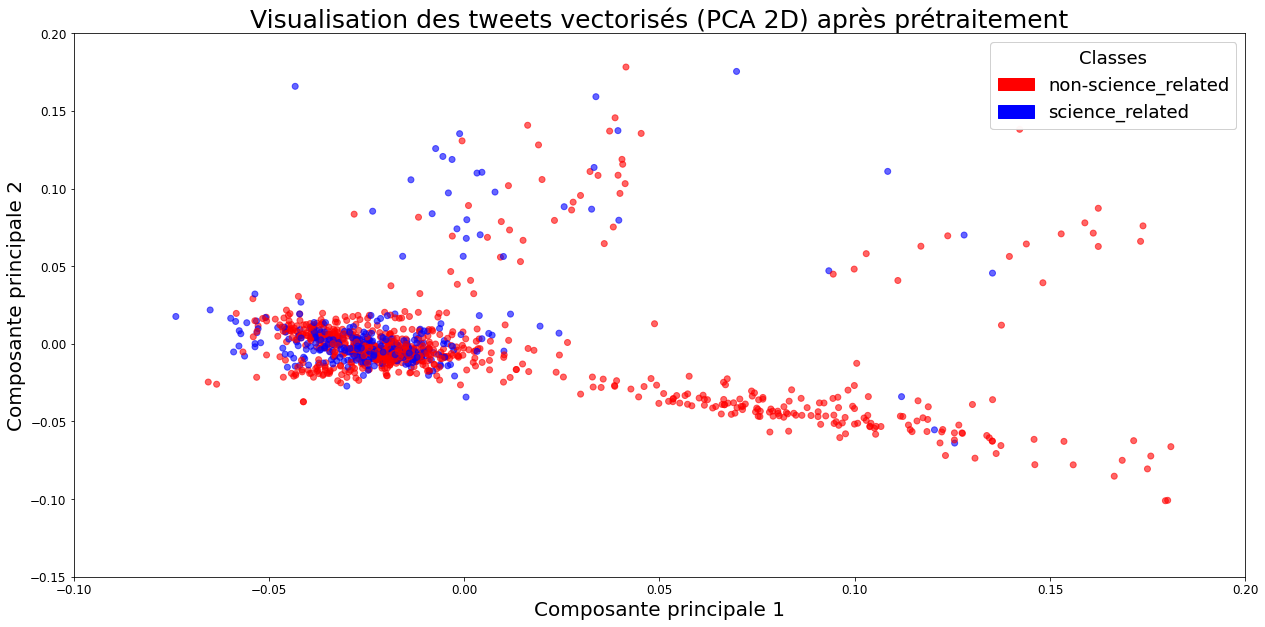
\includegraphics[width=\textwidth]{images/PCA-APT}
    \caption{Visualisation des tweets vectorisés (PCA 2D) après prétraitement}
    \label{fig:pca-apt}
\end{figure}